

% Path to iimage needed for header.
\newcommand\typopath{EconEpsilon}

\documentclass[12pt,a4paper,english,fleqn]{article}
\usepackage{mathptmx}
\usepackage[scaled=0.86]{helvet}
\renewcommand{\familydefault}{\rmdefault}
\usepackage[T1]{fontenc}
\usepackage[latin9]{inputenc}
\usepackage{fancyhdr}
\pagestyle{fancy}
\setcounter{secnumdepth}{2}
\usepackage{graphicx}
\usepackage[authoryear]{natbib}


%Define EconEJ colors
\usepackage{xcolor}
\definecolor{EconomicsGray}{RGB}{198,212,225}
\definecolor{EconomicsLightBlue}{RGB}{127,191,192}
\definecolor{EconomicsBlue}{RGB}{0,63,138}
\definecolor{EconomicsDarkBlue}{RGB}{0,63,117}

% You need this for the headers:
\usepackage{graphicx}

% Headers and footers for Economics E-Journal

\fancyhf{}
\fancyhead[C]{{{\raisebox{-1.5pt}{
\includegraphics[scale=.05]{EconEpsilon}}}\hspace{-.2ex}\small{\hskip -1pt\textcolor{EconomicsDarkBlue}{\textsf{\textbf{conomics}\textmd{~Discussion~Paper}}}}}}

\renewcommand\headrulewidth{0pt}
\renewcommand\headheight{17pt}

\fancyfoot[R]{{\small \sf\thepage}}
\fancyfoot[L]{{\small\sf{{www.economics-ejournal.org}}}}

% Caption formatting
\usepackage[font=footnotesize,labelfont=bf]{caption}


% Reduce font size for section
\makeatletter
\renewcommand\section{\@startsection{section}{1}{\z@}
{-5ex \@plus -1ex \@minus -.2ex}{2.3ex \@plus.2ex}{\normalfont\large\bf}}

%Reduce font size for subsection
\renewcommand\subsection{\@startsection{subsection}{2}
{\z@}{-3.25ex\@plus -1ex \@minus -.2ex}{1.5ex \@plus .2ex}{\normalfont\bf}}


% Enforce proper line breaks and avoid widows and orphans
\tolerance 1414
\hbadness 1414
\emergencystretch 1.5em
\hfuzz 0.3pt
\widowpenalty = 10000
\clubpenalty=10000
\vfuzz \hfuzz
\raggedbottom

%Set date to empty
\date{}

% Format footnotes

% Footnote formatting
\usepackage[hang]{footmisc}
\renewcommand{\hangfootparindent}{1em}
\renewcommand{\hangfootparskip}{0em}
\renewcommand{\footnotemargin}{0.00001pt}
\def\footnotelayout{\hspace{1em}}%

%%%%%%%%%%%%%%%%%%%%%%%%%%%%%%%%%%

% Place your own additions to the preable HERE, that is, BEFORE the following
% call to hyperref

%%%%%%%%%%%%%%%%%%%%%%%%%%%%%%%%%%%

%Hyperlink settings for linkcolors and initial view
\usepackage[%
colorlinks=true,%
linkcolor=black,%
citecolor=black,%
urlcolor=EconomicsDarkBlue,%
pdfstartview=FitH,%
pdfview=FitH,%
pdfpagemode=UseNone]{hyperref}
\hypersetup{pdftitle={Economics: The Open Access, Open Assessment E-Journal}}

% Define font for hyperlinks
\def\UrlFont{\normalfont}

% Some fine-tuning of layout
\usepackage{microtype}

%%%%%%%%%%%%%%%%%%%%%%%%%%%%%%%%%%%

% Put your additions to the preable above the call to hyperref, not here, unless you
% want to modify hyperref settings, as is the case with the precvious two commands

\@ifundefined{showcaptionsetup}{}{%
 \PassOptionsToPackage{caption=false}{subfig}}
\usepackage{subfig}
\AtBeginDocument{
  \def\labelitemi{\tiny\(\bullet\)}
}

\makeatother

\usepackage{babel}

\begin{document}

\title{Here is the Title of Your Paper}


\author{Your name%
\thanks{Give your affiliation and thanks here.%
}.}
\maketitle
\begin{abstract}
\noindent Here comes your abstract.

This is a template for documents prepared with \LaTeX{} for the journal
Economics-The Open Access, Open Assessment E-Journal (www.economics-ejournal.org).

You find further instructions in the Introduction. Please read them.

\noindent \medskip{}


\noindent \emph{Keywords: }Insert the keywords here, separated by
commas.

\noindent \emph{Journal of Economic Literature Classification: }Insert
the classification numbers, such as \ J7, B54,\emph{ }etc. here\emph{.}
\end{abstract}
\noindent \newpage{}


\section{Introduction}

\noindent Here the text of your introduction.

Some further notes:

This template is developed for \LaTeX{}. For proper output you need
to put the the graphic \texttt{EconEpsilon.jpg }either in the folder
containing your active document, or where \LaTeX{} can find it. You
may also point directly to it by adjusting the second line in the
preamble. Currently it is \texttt{\textbackslash{}newcommand\textbackslash{}typopath\{EconEpsilon\}}.
If the file \texttt{EconEpsilon.jpg} is located in \texttt{C:\textbackslash{}Documents\textbackslash{}New},
the line has to be changed into \texttt{\textbackslash{}newcommand\textbackslash{}typopath\{C:/Documents/New/EconEpsilon\},}
for instance. (Note that you have to replace backslashes by slashes
in the path.)

Make sure that you compile with pdflatex. (View and print as PDF,
don't use DVI==>PDF). If it works, save this file under another name
in the same directory. Then play around with it. If it does not work,
check you \LaTeX{} installation.


\section{Here the Title of Your Second Section}

Here your second





 Section, but I insert here some further instructions
instead.

For the bibliography, use the Economics E-Journal style sheet \texttt{EconEJ.bst},
available at \texttt{www.economics-ejournal.org}. This note contains
an example for a bibliographic reference using these files. The reference
to the example bibliography \texttt{EconEJ.bib} is at the bottom of
this file.

Regarding figures and tables, use floats with preferred float placement
on top of page. For figures and sub-figures you see two examples below:
Figure \ref{fig:Example figure} illustrates a simple figure, and
Figure \ref{fig:Subfigures} illustrates a figure with two sub-figures.


\begin{figure}[t]
\centering{}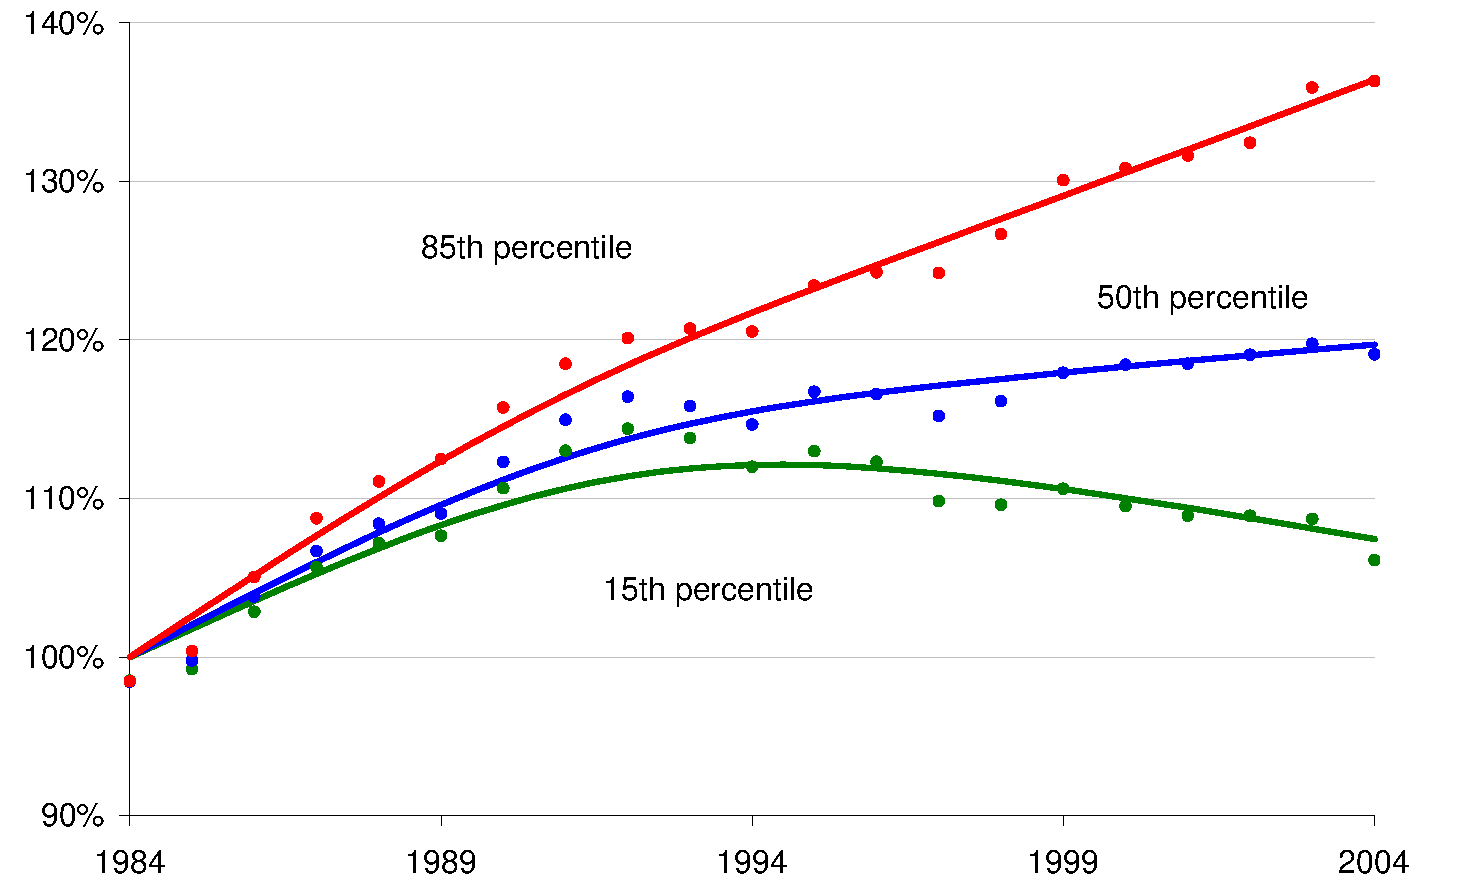
\includegraphics[width=0.8\columnwidth]{percentiles}\caption{\label{fig:Example figure}This is a graphic from \citet{Schlicht07}}
\end{figure}


\begin{figure}[t]
\centering{}\subfloat[Subfigure 1]{\centering{}\includegraphics[width=0.45\columnwidth]{productivitycurve}}\hfill{}\subfloat[Subfigure 2]{

\begin{centering}
\includegraphics[width=0.45\columnwidth]{productivitycurve}
\par\end{centering}

}\caption{\label{fig:Subfigures}This is an example for a float with two subfigures. }

\end{figure}


\bibliographystyle{EconEJ}
\bibliography{EconEJ}

\end{document}
